\section{Question 4}

It is important to consider the limitations of the evaluation undertaken in this report.
Many of the Scottish figures used in the hypothesis and simulation
% (e.g. peak power demand, necessary EES power rating, average winter CF for hydro, mean winter demand, distribution files in EnergyPLAN) 
were based on UK data.
To make a more accurate evaluation, it is important to use accurate data for Scotland, especially for weather data like wind and solar which can vary greatly from region to region \citep{Muller2015}.
Furthermore, it is likely that the upscale of the RE generation mix would need to be more customised to suit Scotland, and not done with a blanket rate \citep{Muller2015}.
Lastly, the evaluation completely ignores the demand for heating, cooling and transport.
With aspirations to make electricity production carbon neutral and subsequently make these other demands electric,
% (such as with electric heating and electric vehicles), 
the electricity demand is expected to grow significantly.

Some strong points of the final optimised scenario were that it was able to reduce the overall demand thanks to DSM and that it was better able to integrate VRE generation.
DSM is an important strategy for optimising our energy use.
As seen, load shifting helps match demand with supply.
Another form of DSM that is necessary in the fight against climate change is strategic conservation, which is essentially demand reduction.
This can be achieved by reducing heating demands in buildings (by making them more airtight and insulated) and by reducing lighting demands (through the use of more energy efficient technology e.g. light-emitting diodes (LEDs)).
However, the level of DSM simulated is currently infeasible in reality; reducing the DSM to a currently feasible level would likely require a larger installed capacity of renewable technologies and EES.
It is also believed that the scenario could have been further optimised to make even more use of the PHS and VRE generation if the author had more time and experience with EnergyPLAN.

Considering that the combined investment cost for the PHS pump and turbine in the optimised scenario is £16.98~billion (see Table~\ref{tbl:EP_PHS_total_costs}), it seems the costs calculated for the hypothetical scenario in terms of GWh were unreasonably large (see Table~\ref{tbl:costs_calc}).
It seems more appropriate to calculate costs in terms of power rating as opposed to storage capacity.

In spite of all that, the scenario simulated in EnergyPLAN was based on a PHS rating of 3.4~GW which Scotland was found to not have the potential for (albeit from what is likely to be incomplete data).
This indicates that in order to achieve 100\% RE generation, stability and independence of the grid, there needs to be a more diversified form of EES and/~or interconnects.

As was found with Scotland, it can be assumed that most countries do not have enough resources to make their grids completely independent if operating with 100\% RE.
Therefore, these grids cannot not be viewed as independent entities and interconnects should be encouraged (as the Siemens case study recommended).
% to form international grid stability solutions.
For example, the UK and Europe depend on Scotland as a major source of wind and hydro generation.
And Scotland has plenty of wind electricity to export but not enough EES capacity to store it.
Hence, both sides can benefit from interconnects \citep{Muller2015}.

\begin{wrapfigure}{r}{0.4\textwidth}
	\centering
	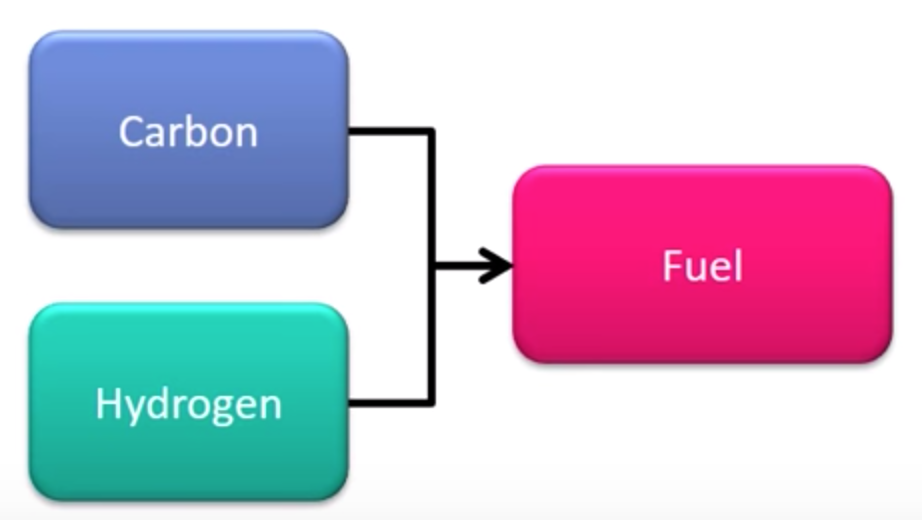
\includegraphics[width=0.4\textwidth]{figures/electrofuels.png}
	\rule{0.4\textwidth}{0.5pt} % use line???
	\caption{Electrofuel concept \citep{Electrofuels2016}.}
	\label{fig:electrofuels}
\end{wrapfigure}

Diversification of EES forms seems necessary to achieve 100\% RE generation.
One form that is comparable to PHS in magnitude is compressed air energy storage (CAES), but it maintains the use of natural gas and requires suitable geological sites or high capital investments.
Much like it is beneficial to view grids as interconnected networks, it is beneficial to view electricity as connected to other demand sectors, notably heating and transport.
Current research shows that electricity can easily, inexpensively and reliably be stored as a liquid or gas fuel which can then be used to supply heating and/ or transport demands.
Sterner calls this Power-to-Gas (see Figure~\ref{fig:p2g}) and Connolly talks about creating and using electrofuels (see Figure~\ref{fig:electrofuels}) \citep{Sterner2017, Electrofuels2016}.
Electrofuels are synthetic fuels that are suitable for trucks, aviation and ships.
They can be created through a combination of carbon and hydrogen; the carbon can come from emissions from power plants, bioenergy or even industry, and the hydrogen would be produced by electricity via electrolysis.
In both Power-to-Gas and electrofuels, excess VRE generation can be stored to help supply other major demands and not just electrical demands.

\begin{figure}[htbp]
	\centering
	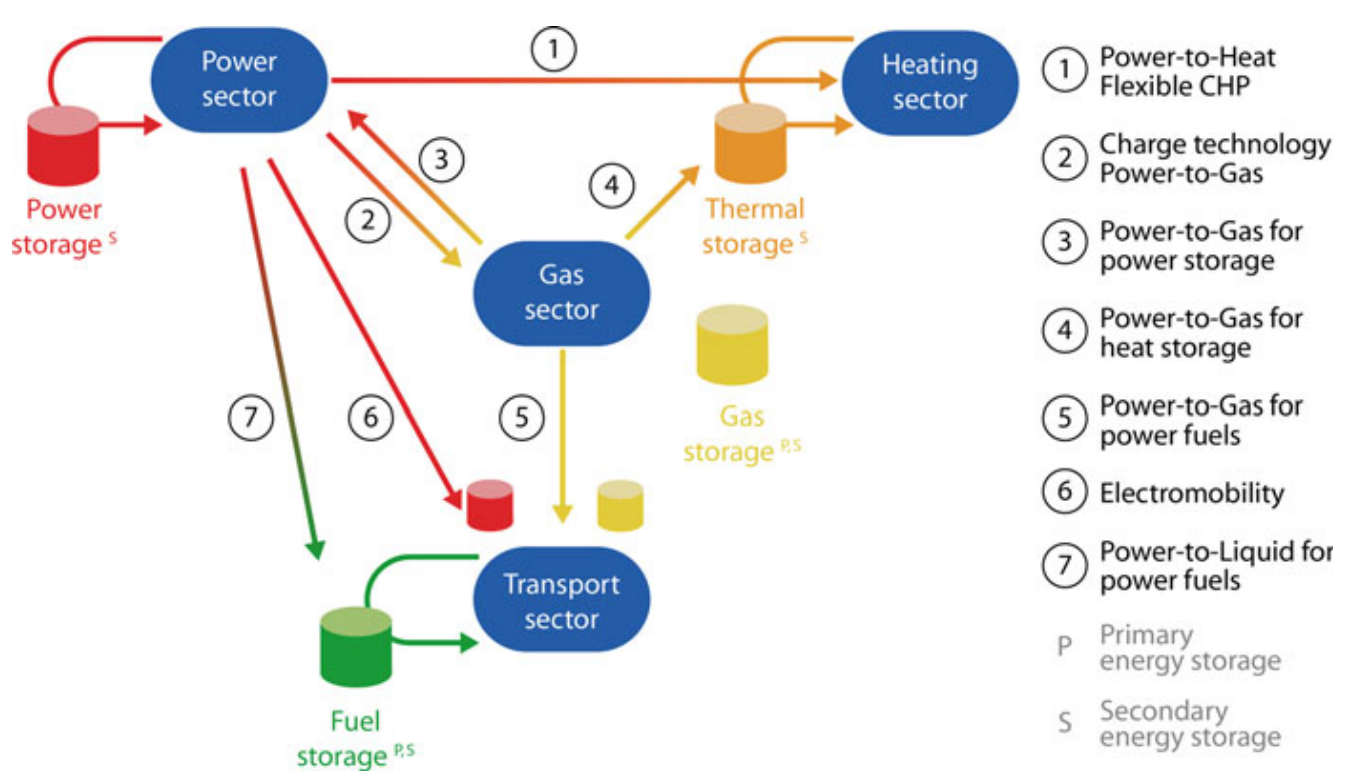
\includegraphics[width=0.9\textwidth]{figures/p2g.png}
	\rule{\textwidth}{0.5pt} % use line???
	\caption{Power-to-Gas storage concept \citep[p.~2781]{Sterner2017}.}
	\label{fig:p2g}
\end{figure}

% MIA: I did not do much for Q4 really, I just talk about it lot. also saying if I would have EES storage in form of CAES it would be this much, flywheels this etc.

%Q1: (However, it should be noted that there might be discrepancies between hydro's capacity factors in the UK and Scotland.)
%accurate data for Scotland: demand, wind, solar

%Interconnects are necessary; cannot view national grids as independent entities.
%Scotland does not seem to have the PHS potential to meet peak demand.
%UK depends on Scotland as major source of wind and hydro generation.
%UK is part of a larger European solution of grid stability.

%Should not scale up RE generation mix equally across technologies; some technologies are more reliable and/ or fruitful than others.

%just elec